% Prof. Dr. Ausberto S. Castro Vera
% UENF - CCT - LCMAT - Curso de Ci\^{e}ncia da Computa\c{c}\~{a}o
% Campos, RJ,  2022
% Disciplina: Paradigmas de Linguagens de Programa\c{c}\~{a}o
% Aluno: Ricardo Willian Pontes da Silva


\chapter{Ferramentas existentes e utilizadas}
Neste capítulo será apresentadas algumas ferramentas para auxiliar no desenvolvimento utilizando a linguagem de programação Python, algumas dessas ferramentas foram utilizadas até mesmo para realizar esse trabalho. As ferramentas a seguir terão as \begin{itemize}
	\item Nome da ferramenta
	\item Versão atual e utilizada
	\item Descrição e informações
	\item Telas capturadas da ferramenta
	\item Endereço na Internet
\end{itemize}

    \section{Visual Studio Code}

O Visual Studio Code é um ambiente de desenvolvimento poderoso para a linguagem Python por meio dos seus recursos e cargas de trabalho de ciência de dados. Com a utilização do Visual Studio para a criação de códigos com a linguagem Python a aprendizagem se torna de fácil acesso e gratuita com diversas bibliotecas disponíveis no seu ambiente. Com a união dessas ferramentas, é possível criar aplicativos Web, serviços Web, aplicativos de desktop, scripts e computação científica no Visual Studio, podendo ser utilizados por cientistas e desenvolvedores profissionais e casuais.\\
  \begin{figure}[H]
	\begin{center}
		\caption{Ambiente de desenvolvimento no Visual Studio} \label{ling1}
		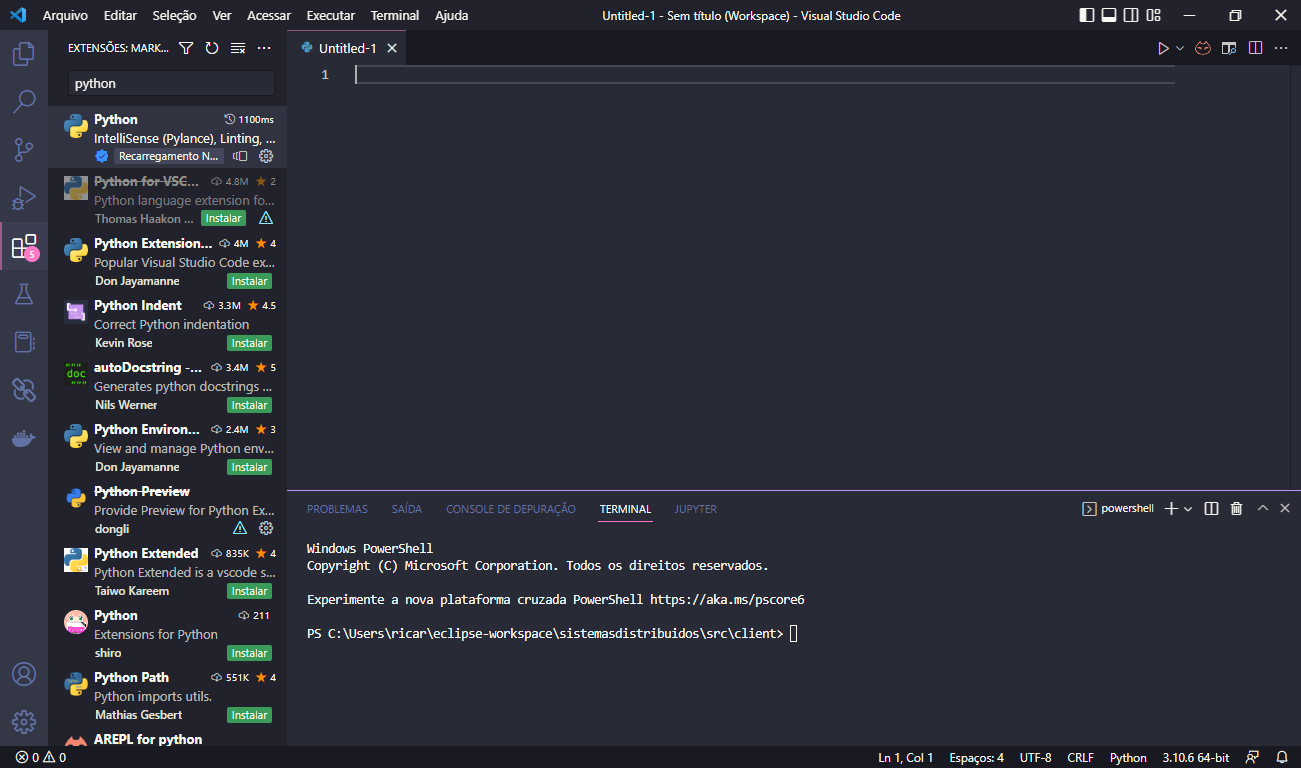
\includegraphics[width=15cm]{visualStudioPy.PNG} \\
		{\tiny \sf Fonte:{ Autor}}
	\end{center}
\end{figure}
A ferramenta Visual Studio é permissiva o desenvolvimento de N linguagens de programação e afins, desta forma, para utilizá-la para a linguagem Python é necessário selecionar e baixar no dispositivo as extensões necessárias para a mesma, como mostrado na figura acima. Atualmente o Visual Studio se encontra na versão 17.4 podendo ser utilizado também versões ainda em desenvolvimento.

    \section{Compilador XYZ}


    \section{Interpretador UVW}


    \section{Ambientes de Programa\c{c}\~{a}o IDE MNP} 